% --------------------------------------------------------------------------------

\newpage

\begin{exercise}

Alternative Algorithmen zur Bestimmung minimaler Spannbäume.
Nachfolgend sind die Pseudocodes von drei verschiedenen Algorithmen angegeben.
Alle drei erhalten als Eingabe einen zusammenhängenden kantenbewerteten Graphen und geben eine Kantenmenge $T$ zurück.
Beweisen oder widerlegen Sie für jeden der drei Algorithmen die Behauptung, dass $T$ in jedem Fall ein minimaler Spannbaum ist.

\begin{algorithmic}
    \State Maybe-MST-A($G, w$)
    \State sortiere die Kanten in nichtsteigender Reihenfolge nach ihren Gewichten $w$
    \State $T := E$
    \For{$e \in E$ (in der soeben berechneten Reihenfolge)}
        \If{$T \setminus \Bbraces{e}$ ist ein zusammenhängender Graph}
            \State $T := T \setminus \Bbraces{e}$
        \EndIf
    \EndFor
    \State \Return $T$
\end{algorithmic}

\begin{algorithmic}
    \State Maybe-MST-B($G, w$)
    \State $T := \emptyset$
    \For{$e \in E$ (in einer beliebigen Reihenfolge)}
        \If{$T \cup \Bbraces{e}$ kreisfrei}
            \State $T := T \cup \Bbraces{e}$
        \EndIf
    \EndFor
    \State \Return $T$
\end{algorithmic}

\begin{algorithmic}
    \State Maybe-MST-C($G, w$)
    \State $T := \emptyset$
    \For{$e \in E$ (in einer beliebigen Reihenfolge)}
        \State $T := T \cup \Bbraces{e}$
        \If{$T$ enthält einen Zyklus $c$}
            \State sei $e_0$ eine Kante von $c$ mit maximalem Gewicht
            \State $T := T \setminus \Bbraces{e_0}$
        \EndIf
    \EndFor
    \State \Return $T$
\end{algorithmic}

\end{exercise}

% --------------------------------------------------------------------------------

\begin{solution}

\phantom{}

\begin{enumerate}[label = (\Alph*)]

    \item Der Algorithmus von Kruskal startet leer und bezieht nur die nötigsten Kanten (d.h. jene mit minimalen Kosten) in den potentiellen MST mit ein.
    Unser Algorithmus startet jedoch voll und entfernt die \Quote{unnötigsten} Kanten (d.h. jene mit maximalen Kosten) von dem potentiellen MST.

    Die Vermutung, dass Letzterer korrekt ist, klingt daher durchaus plausibel.
    Um dies zu beweisen, orientieren wir uns entsprechend am Beweis von Satz 7.2.

    Sei $e_1, \dots, e_n$ eine Sortierung von $E$, so dass $c(e_1) \geq \cdots \geq c(e_n)$, sei $E_0 = \emptyset$ und

    \begin{align*}
        E_{i+1}
        =
        \begin{cases}
            E_i \setminus \Bbraces{e_{i+1}} & \text{falls}~ (V, E_i \setminus \Bbraces{e_{i+1}}) ~\text{zusammenhängenden ist und} \\
            E_i                             & \text{sonst.}
        \end{cases}
    \end{align*}

    Der Algorithmus antwortet mit $(V, E_n)$.

    \textit{Beweis.}
    Zunächst ist klar, dass $B = (V, E_n)$ zusammenhängend ist.
    $B$ ist aber auch zyklenfrei:
    Angenommen, $B$ wäre nicht zyklenfrei, sei $e_{i_1}, \dots, e_{i_k} \in E_n$ ein Zyklus in $B$.
    $e_{i_1}, \dots, e_{i_k}$ wurden vom Algorithmus nicht entfernt, also waren $(V, E_{i_1 - 1} \setminus \Bbraces{e_{i_1}}), \dots, (V, E_{i_k - 1} \setminus \Bbraces{e_{i_k}})$ nicht zusammenhängend.
    Sei $\ell = 1, \dots, k$.
    Weil nun $E_{i_\ell - 1} \setminus \Bbraces{e_{i_\ell}} \supset E_n \setminus \Bbraces{e_{i_\ell}}$, wäre somit aber $(V, E_n \setminus \Bbraces{e_{i_\ell}})$ ebenso nicht zusammenhängend.
    Aus dem Zyklus $e_{i_1}, \dots, e_{i_k} \in E_n$ darf man aber eine beliebige Kante löschen und der resultierende Graph $(V, E_n \setminus \Bbraces{e_{i_\ell}})$ wäre noch immer zusammenhängend.
    Widerspruch!

    Für die Minimalität von $B$ reicht es zu zeigen, dass für alle $i \in \Bbraces{0, \dots, n}$ ein minimaler Spannbaum von $G$ mit Kantenmenge $M_i$ existiert so dass $E_i \supseteq M_i$.
    Dann ist nämlich $E_n = M_n$ und damit $B$ minimal.

    Wir gehen mit Induktion nach $i$ vor.
    Der Fall $i = 0$ ist trivial.
    Für den Induktionsschritt definieren wir $M_{i+1} = M_i$ falls keine Kante weggenommen wird oder die weggenommene Kante $e_{i+1} \not \in M_i$.
    Sei nun also $E_{i+1} = E_i \setminus \Bbraces{e_{i+1}}$, $(V, E_{i+1})$ zusammenhängend und $e_{i+1} \in M_i$.
    Weil $(V, M_i)$ als Baum minimal zusammenhängend ist, ist $(V, M_i \setminus \Bbraces{e_{i+1}})$ nicht mehr zusammenhängend.
<<<<<<< HEAD
    Weil $E_{i+1}$ zusammenhängend ist, können die beiden ZHKs von $(V, E_i \setminus \Bbraces{e_{i+1}}) \supseteq (V, M_i \setminus \Bbraces{e_{i+1}}) = (V, E_{i+1})$ durch ein $e_j \in E_{i+1}$ verbunden werden. 
    Dabei ist $e_{i+1} \neq e_j \in E_{i+1} = E_i \setminus \Bbraces{e_{i+1}}$.
    Ebenso ist $e_j \not \in M_i \setminus \Bbraces{e_{i+1}}$, weil die ZHKs sonst bereits verunden gewesen wären.
=======
    Weil $E_{i+1}$ zusammenhängend ist, können die beiden Zusammenhangskomponenten von
    $(V, M_i \setminus \Bbraces{e_{i+1}}) \subseteq (V, E_i \setminus \Bbraces{e_{i+1}}) = (V, E_{i+1})$
    durch ein $e_j \in E_{i+1}$ verbunden werden mit $e_j \neq e_{i+1}$.
    Ebenso ist $e_j \not \in M_i \setminus \Bbraces{e_{i+1}}$, weil die Zusammenhangskomponenten sonst bereits verbunden gewesen wären.
>>>>>>> b97c5c8db51b80b26a521fa55f79d1dc32d83e29
    Daher muss $e_j \not \in M_i$. (Oder: Da $(V,E_{i + 1})$ zusammenhängend ist muss $e_{i + 1}$ aus einem Zykel $z$ von $(V,E_i)$ stammen. Außerdem ist $M_i$ zyklenfrei und da $e_{i + 1} \in M_i$ muss es schon ein $e_j$ aus $z$ geben mit $e_j \notin M_i$.)

    \begin{align*}
        M_{i+1}
        :=
        (
            \underbrace
            {
                \underbrace{M_i}_{\subseteq E_{i+1}}
                \setminus
                \Bbraces{e_{i+1}}
            }_{
                \subseteq E_{i+1}
            }
        )
        \dot \cup
        \underbrace
        {
            \Bbraces{e_j}
        }_{
            \subseteq E_{i+1}
        }
        \subseteq
        E_{i+1}
    \end{align*}

    $(V, M_{i+1})$ ist also zusammenhängend.

    Weiters ist $|M_{i+1}| = |M_i| = |V| - 1$ da ja $e_j \notin M_i$ und $e_{i+1} \in M_i$ ist und $(V, M_{i+1})$ mit Satz 2.3 also ein Spannbaum von $G$.

    Außerdem ist $c(e_j) \leq c(e_{i+1})$, denn $c(e_j) > c(e_{i+1})$ impliziert $j < i + 1$ und damit $j-1 < j \leq i < i+1$.
    Weil die $E$-Kantenmengen monoton nicht-steigen, heißt das $E_{j-1} \supseteq E_j \supseteq E_i \supseteq E_{i+1}$.

    \begin{align*}
        \implies
        E_{j-1} \setminus \Bbraces{e_j}
        \stackrel{!}{\neq}
        E_j
        \supseteq
        E_{i+1}
        \ni
        e_j
    \end{align*}

    Laut Konstruktion, und weil $e_j \not \in M_i$, wäre dann aber

    \begin{multline*}
        (V, E_{j-1} \setminus \Bbraces{e_j}) ~\text{nicht zusammenhängend}~
        \supseteq
        (V, E_i     \setminus \Bbraces{e_j}) ~\text{nicht zusammenhängend} \\
        \supseteq
        (V, M_i     \setminus \Bbraces{e_j}) ~\text{nicht zusammenhängend}~
        =
        (V, M_i)                             ~\text{nicht zusammenhängend.}
    \end{multline*}

    Widerspruch!
    Also ist $c(M_{i+1}) \leq c(M_i)$ und, da $M_i$ minimal ist, $c(M_{i+1}) = c(M_i)$ und $M_{i+1}$ also ebenfalls ein minimaler Spannbaum.

    Q.E.D.

    \item Maybe-MST-B ist genau der Algorithmus von Kruskal ohne Sortierung.

    \includegraphicsboxed{DGA/DGA - Algorithmus von Kruskal.png}

    Ohne Sortierung wird es aber schwer.
    Dazu betrachten wir ein Dreieck mit einer bösen Kanten-Reihenfolge.

    \begin{align*}
        E := [e_1, e_2, e_3],
        \quad
        c(e_1) > c(e_2) > c(e_3)
    \end{align*}

    \begin{center}
        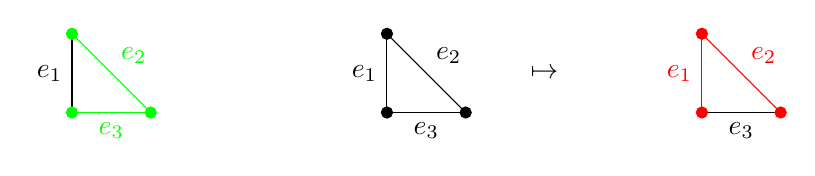
\begin{tikzpicture}

    \begin{scope}[xshift = -4 cm]
        
        \coordinate (v_1) at (0, 0);
        \coordinate (v_2) at (1, 0);
        \coordinate (v_3) at (0, 1);

        \draw [color = green] (v_1) -- node [below]       {$e_3$} (v_2);
        \draw [color = green] (v_2) -- node [above right] {$e_2$} (v_3);
        \draw [color = black] (v_3) -- node [left]        {$e_1$} (v_1);

        \filldraw [color = green] (v_1) circle (2pt);
        \filldraw [color = green] (v_2) circle (2pt);
        \filldraw [color = green] (v_3) circle (2pt);

    \end{scope}

    \draw (-2, 0.5) node {$\mapsfrom$};

    \begin{scope}
        
        \coordinate (v_1) at (0, 0);
        \coordinate (v_2) at (1, 0);
        \coordinate (v_3) at (0, 1);

        \draw [color = black] (v_1) -- node [below]       {$e_3$} (v_2);
        \draw [color = black] (v_2) -- node [above right] {$e_2$} (v_3);
        \draw [color = black] (v_3) -- node [left]        {$e_1$} (v_1);

        \filldraw [color = black] (v_1) circle (2pt);
        \filldraw [color = black] (v_2) circle (2pt);
        \filldraw [color = black] (v_3) circle (2pt);

    \end{scope}

    \draw (2, 0.5) node {$\mapsto$};

    \begin{scope}[xshift = 4 cm]
        
        \coordinate (v_1) at (0, 0);
        \coordinate (v_2) at (1, 0);
        \coordinate (v_3) at (0, 1);

        \draw [color = black] (v_1) -- node [below]       {$e_3$} (v_2);
        \draw [color = red]   (v_2) -- node [above right] {$e_2$} (v_3);
        \draw [color = red]   (v_3) -- node [left]        {$e_1$} (v_1);

        \filldraw [color = red] (v_1) circle (2pt);
        \filldraw [color = red] (v_2) circle (2pt);
        \filldraw [color = red] (v_3) circle (2pt);

    \end{scope}

\end{tikzpicture}
    \end{center}

    Der linke (grüne) Spannbaum hat $B_\mathrm{l}$ geringere Kosten als der rechte (rote) $B_\mathrm{r}$.

    \begin{align*}
        c(B_\mathrm{l})
        =
        c(e_2) + c(e_3)
        <
        c(e_1) + c(e_2)
        =
        c(B_\mathrm{r})
    \end{align*}

    \item Sei $E = [e_1, \dots, e_n]$ eine beliebige Kanten-Reihenfolge.
    Der gegebene Algorithmus operiert wie folgt.

    \begin{align*}
        E_0 := \emptyset,
        \quad
        E_{i+1}
        :=
        \begin{cases}
            (E_i \cup \Bbraces{e_{i+1}}) \setminus \Bbraces{e_{i_1}},
            &
            \Exists (e_{i_1}, \dots, e_{i_k}) ~\text{Zyklus}~ \subset (V, E_i \cup \Bbraces{e_{i+1}}): \\
            &
            c(e_{i_1}) \geq c(e_{i_2}), \dots, c(e_{i_k}), \\
            E_i \cup \Bbraces{e_{i+1}}, & \text{sonst}
        \end{cases}
    \end{align*}

    Der Algorithmus antwortet mit $(V, E_n)$.

    Um die Korrektheit des Algorithmus zu beweisen, brauchen wir zunächst ein Lemma.

    \textbf{Lemma.}
    Sei $G = (V, E)$ ein endlicher, zyklenfreier Graph.
    Sei $e$ eine Kante, sodass $G^\prime = (V, E \cup \Bbraces{e})$ einen Zyklus enthält.
    Dann enthält $G^\prime$ höchstens (d.h. genau) einen Zyklus.

    \textit{Beweis.}
    Angenommen, $G^\prime$ enthielte $2$ verschiedene Zyklen $a = (a_1, \dots, a_n)$ und $b = (b_1, \dots, b_m)$.
    Offenbar muss $e \in a$, da sonst $a$ Zyklus von $G$ wäre.
    Dasselbe gilt für $b \ni e$.
    Nun können wir aber aus $a \setminus e$ und $b \setminus e$ einen Zyklus von $G$ erzeugen.
    Widerspruch!

    Q.E.D.

    \textbf{Bemerkung.}
    Wenn man aus einem Graphen (z.B. $G^\prime$ aus dem obigen Lemma), der genau einen Zyklus besitzt eine Zyklus-Kante löscht, dann ist der resultierende Graph zyklenfrei.

    \textit{Beweis (Korrektheit von Maybe-MST-C).}
    Laut dem obigen Lemma und der Bemerkung, ist klar, dass $B = (V, E_n)$ zyklenfrei ist.
    $B$ ist aber auch zusammenhängend:

    Sei $i = 1, \dots, n$ und verbinde $e_{i+1}$ zwei ZHKs $Z_1, Z_2 \subseteq (V, E_i)$.
    Wir behaupten, dass $(V, E_i \cup \Bbraces{e_{i+1}})$ zyklenfrei ist.
    Laut dem obigen Lemma und der Bemerkung, ist nämlich klar, dass $(V, E_i)$ zyklenfrei ist.
    Daher sind insbesondere die ZHKs (Bäume) $Z_1$ und $Z_2$ zyklenfrei.
    $Z := Z_1 \cup \Bbraces{e_i} \cup Z_2 \subseteq (V, E_i \cup \Bbraces{e_{i+1}})$ ist also auch zyklenfrei.
    $(V, E_i \cup \Bbraces{e_{i+1}})$ ist also insgesamt Zyklenfrei.
    Der Algorithmus entscheidet sich also für $E_{i+1} = E_i \cup \Bbraces{e_{i+1}}$.
    Zusammenfassend:
    Wenn $e_{i+1}$ zwei ZHKs verbindet wird $e_{i+1}$ vom Algorithmus nicht entfernt.

    Wir zeigen mit Induktion, dass es immer, d.h. im $i$-ten Schritt, genug Kanten $\in \Bbraces{e_i, \dots, e_n}$ gibt, sodass alle ZHKs von $(V, E_{i-1})$ verbunden werden können.
    Der Induktionsanfang ist klar, weil $G = (V, E)$ zusammenhängend ist und die ZHKs von $(V, E_0)$ genau die Singleton-Graphen $(\Bbraces{v}, \emptyset)$, $v \in V$ sind.
    Für den Induktionsschritt gebe es solche Kanten im $i$-ten Schritt.
    Wenn keine der Kanten darin verwendet wurde, gibt es alle davon auch im $(i+1)$-ten Schritt wieder.
    Wenn eine ($e_i$) verwendet wurde, dann wurde sie laut den oberen Überlegungen nicht vom Algorithmus aus $E_i \cup \Bbraces{e_i}$ entfernt.
    Weil dann aber gerade zwei ZHKs von $(V, E_{i-1})$ verbunden wurde, gibt es in $(V, E_i)$ dann aber genau eine ZHK weniger.
    Die im $i$-ten Schritt verwendete Kante $e_i$ wird daher im $(i+1)$-ten (bis $n$-ten) Schritt garnicht mehr gebraucht, um diese Bereiche im Graphen zu verbinden, weil sie ja bereits, vermöge $e_i$ zusammenhängen.

    Der Algorithmus arbeitet alle Kanten $\in E$ ab, also auch all jene, die ZHKs verbinden.
    Der resultierende Graph $B$ ist daher zusammenhängend.

    Wir müssen also nur noch zeigen, dass $B$ minimal ist unter allen Spannbäumen.
    Dazu, reicht es zu zeigen, dass

    \begin{align*}
        \Forall i = 1, \dots, n:
        \Forall G_Z = (V_Z, E_Z) ~\text{ZHK von}~ (V, \bar E_i):
        (V_Z, E_Z \cap E_i) \subset ~\text{MST von}~ G_Z.
    \end{align*}

    Dabei sei $\bar E_i := \Bbraces{e_1, \dots, e_n}$ die Menge der Kanten, die der Algorithmus bis zum $i$-ten Schritt \Quote{gesehen} hat.
    Weil ja $G = (V, E)$ zusammenhängend ist, hat $G$ nur eine ZHK (sich selbst).
    Weil $\bar E_n = E$, steht für $i = n$ die Behauptung oben praktisch schon da.
    Wir führen Induktion nach dem $i$-ten Schritt.
    Der Induktionsanfang $i = 0$ ist trivial.

    Für den Induktionsschritt unterscheiden wir $2$ Fälle.

    \begin{enumerate}[label = \arabic*.]

        \item Fall ($e_{i+1}$ verbindet $2$ ZHK von $(V, \bar E_i$)):
        
        Seien $Z_1 = (V_{Z_1}, E_{Z_1})$ und $Z_2 = (V_{Z_2}, E_{Z_2})$ jene ZHKs.

        \begin{align*}
            Z := (V_Z, E_Z) = (V_{Z_1} \cup V_{Z_2}, E_{Z_1} \cup E_{Z_2} \cup \Bbraces{e_{i+1}})
        \end{align*}

        $Z$ ist eine ZHK von $(V, \bar E_{i+1})$.

        $e_{i+1}$ ist die einzige Verbindung zwischen $Z_1$ und $Z_2$.
        Jeder ST $T$ von $Z$ muss durch $Z_1$ und $Z_2$.
        Also muss $T$ auch durch $e_{i+1}$ gehen, weil sonst wäre $T$ nicht zusammenhängend.

        \begin{align*}
            \stackrel
            {
                \mathrm{IV}
            }{\implies}
            & \tilde M_1 := (V_{Z_1}, E_i \cap E_{Z_1}) \subseteq M_1 ~\text{MST von}~ Z_1, \\
            & \tilde M_2 := (V_{Z_2}, E_i \cap E_{Z_2}) \subseteq M_2 ~\text{MST von}~ Z_2
        \end{align*}

        Sei $M$ MST von $Z$, dann sind $M_1, M_2 \subseteq M$.

        \begin{align*}
            \implies
            \tilde M_1, \tilde M_2 \subseteq M,
            \quad
            e_{i+1} \in M
        \end{align*}

        \begin{align*}
            \implies
            (V_Z, E_{i+1} \cap E_Z)
            & =
            (V_{Z_1} \cup V_{Z_2}, (E_i \cap (E_{Z_1} \cup E_{Z_2})) \cup \Bbraces{e_{i+1}}) \\
            & =
            (V_{Z_1} \cup V_{Z_2}, (E_i \cap E_{Z_1}) \cup (E_i \cap E_{Z_2})) \cup \Bbraces{e_{i+1}}) \\
            & =
            \tilde M_1 \cup \tilde M_2 \cup_\mathrm{Kanten} \Bbraces{e_{i+1}} \\
            & \subseteq
            M
        \end{align*}

        Für die restlichen ZHKs (außer $Z$) kann man die IV anwenden.

        \item Fall ($e_{i+1}$ verbindet $2$ Knoten $\in$ ZHK von $(V, \bar E_i$)):
        
        Sei $Z = (V_Z, E_Z)$ jene ZHK.
        
        \begin{enumerate}[label = 2.\arabic*.]

            \item Fall ($(V, E_i \cup \Bbraces{e_{i+1}})$ hat einen Zyklus):
            
            Sei $z = (e_{i_1}, \dots, e_{i_k}) \subseteq (V_, E_i \cup \Bbraces{e_{i+1}}$ jener Zyklus und $c(e_{i_1}) \geq c(e_{i_2}), \dots, c(e_{i_k})$.
            Der Zyklus entsteht dort, wo $e_{i+1}$ hinzugefügt wurde.
            Weil $Z$ als ZHK zusammenhängend ist, ist $e_{i+1} \in z \subseteq (V_Z, E_Z \cap (E_i \cup \Bbraces{e_{i+1}}))$.
            Der Algorithmus entscheidet sich also für $E_{i+1} = (E_i \cup \Bbraces{e_{i+1}}) \setminus \Bbraces{e_{i_1}}$.

            \begin{enumerate}[label = 2.1.\arabic*.]

                \item Fall ($i_1 = i+1$):
                
                \begin{align*}
                    \implies
                    E_{i+1}
                    =
                    (E_i \cup \Bbraces{e_{i+1}}) \setminus \Bbraces{e_{i+1}}
                    =
                    E_i
                \end{align*}

                $Z^\prime := Z \cup_\mathrm{Kanten} \Bbraces{e_{i+1}}$ ist eine ZHK von $(V, \bar E_{i+1})$
                Der MST von $Z \subseteq (V, \bar E_i)$ ist derselbe wie der von $Z^\prime$.
                Die IV ist also direkt anwendbar.

                \item Fall ($i_1 \neq i+1$):
                
                \begin{align*}
                    \implies
                    c(i_1) \geq c(i+1)
                \end{align*}

                Der MST $M_i$ von $(V_Z, E_Z \cap \bar E_i)$ aus der IV verläuft entlang den Kanten $z \setminus \Bbraces{e_{i+1}} \subseteq (V, E_i)$.
                Der MST $M_{i+1}$ von $(V_{Z^\prime}, E_{Z^\prime} \cap \bar E_{i+1})$ verläuft genau gleich, bloß durch die billigere Kante $e_{i+1}$ statt der teureren $e_{i_1}$.

            \end{enumerate}

            \item Fall ($(V, E_i \cup \Bbraces{e_{i+1}})$ ist zyklenfrei):
            
            Der Algorithmus entscheidet ist daher für $E_{i+1} = E_i \cup \Bbraces{e_{i+1}}$.

            \begin{align*}
                \implies
                (V, E_{i+1}) ~\text{zyklenfrei}~
                \implies
                (V_Z, E_Z \cap E_{i+1}) ~\text{zyklenfrei}
            \end{align*}

            Weil $Z$ als ZHK zusammenhängend ist, gehört $e_{i+1}$ zu einem Zyklus $z_1 = (e_{i_1}, \dots, e_{i_k})$.
            Sei $e_{i_\ell} \in E_Z \cap (\bar E_i \setminus E_i)$ eine, von dem Algorithmus weggeschnittene, Kante.
            $e_{i_\ell}$ wurde weggeschnitten, weil sie maximale Kosten in einem, von $z$ verschiedenen Zyklus $z^\prime \subseteq (V, E_{i_\ell - 1} \cup \Bbraces{e_{i_\ell}})$ hatte.
            $z^\prime$ grenzt an $1$ (sogar $2$) Knoten $\in V_Z$ an.
            Weil $Z$ als ZHK zusammenhängend ist, ist $z^\prime \subseteq Z$ ganz in $Z$ enthalten.
            $z_2$ bildet nun wieder einen Zyklus.

            \begin{align*}
                z_2
                :=
                (z_1      \setminus \Bbraces{e_{i_\ell}})
                \cup
                \underbrace
                {
                    (z^\prime \setminus \Bbraces{e_{i_\ell}})
                }_{
                    \subseteq (V_Z, E_Z \cap E_{i_\ell - 1})
                }
                =
                (z_1 \cup z^\prime) \setminus \Bbraces{e_{i_\ell}}
            \end{align*}

            Es kann nun sein, dass der Austausch von $e_{i_\ell}$ mit dem Umweg $z^\prime \setminus \Bbraces{e_{i_\ell}}$ weitere Kanten liefert, die wiederum ausgetauscht werden müssen (und wieder, \dots, und wieder).
            Die Umwege für den Austausch liegen aber in Graphen, mit immer weniger Kanten.
            Insofern sind die $z_1, z_2, \dots$ strikt halbgeordnet (durch $(H, \subsetneq)$).
            (Fun Fact: Das Hasse-Diagrmm dieser HO ist sogar ein Baum mit Wurzel $z_1$.)

            Gegebenenfalls wenden wir auf $z_2$ also dasselbe Argument wie auf $z_1$ an (und wieder, \dots, und wieder).
            Weil $G$ endlich ist, gibt es nur endlich viele verschiedene Zyklen.
            Daher ist insbesondere die Halbordnung $H$ endlich.

            Irgendwann bekommen wir also einen Zyklus $z_\infty$, der nur nicht-weggeschnittene Kanten, d.h. $\in E_Z \cap E_{i+1}$ hat, d.h. minimales Element von $H$ ist.
            Das ist ein Widerspruch dazu, dass $(V_Z, E_Z \cap E_{i+1})$ zyklenfrei ist!

        \end{enumerate}

    \end{enumerate}

    Q.E.D.

    \begin{comment}
    Wir behaupten also, dass $G_n:=(V,E_n)$ ein minimaler Spannbaum ist. Wir arbeiten alle Eigenschaften ab.
    \begin{enumerate}

        \item $G_n$ ist zyklenfrei.
        Dies folgt aus obiger Bemerkung.

        \item Angenommen $G_n$ wäre nicht zusammenhängend.
        Betrachten wir also zwei Zusammenhangskomponeneten $Z_1$ und $Z_2$ dieses Graphen.
        Das heißt aus jedem Pfad der $Z_1$ und $Z_2$ verbindet wird eine Kante durch den Algorithmus gelöscht.
        Wir betrachten einen Zeitpunkt, zu dem nur mehr ein Pfad intakt ist.
        Jede Kante in diesem Pfad kann dann aber nicht mehr in einem Zykel vorkommen, also auch nicht gelöscht werden, ein Widerspruch!

        \item Die Frage ist:
        Ist dieser Spannbaum auch wirklich minimal??

    \end{enumerate}
    \end{comment}

\end{enumerate}

\end{solution}

% --------------------------------------------------------------------------------
